\section{Diskussion}
Für die Bragg-Bedingung ist eine minimale Abweichung von $0,36\%$ vorhanden, dies könnte möglicherweise
unsere Messdaten verfälscht haben wie in der Messereihe zum Emissionsspektrum der Cu-Röntgenröhre.
In der Tabelle (\ref{tab:3}) sind die Abweichungen der Absorptionsenergien aufgelistet.
\begin{table}
  \centering
  \caption{Vergleich von gemessenen Werten mit Literaturwerten.}
  \label{tab:3}
  \begin{tabular}{c c c c}
    \toprule
     & $E_{mes}\,/ \, \text{keV}$  & $E_{lit}\,/ \, \text{keV}$ & $Abweichung \,/\,\%$ \\
    \midrule
    Br & 13,47 & 13,38 & 0,67\\
    Sr & 16,10 & 15,99 & 0,68\\
    Zr & 17,99 & 17,40 & 3,28\\
    \bottomrule
  \end{tabular}
\end{table}
Ein möglicher Grund für die Abweichungen könnte durch nicht genau Winkeleinzeichung im Graphen entstanden worden sein.

Für die Abschirmkonstanten sind die Messwerte und die zugehörigen Abweichungen in der Tabelle
\ref{tab:4} dargestellt.

\begin{table}[H]
  \centering
  \caption{Vergleich von gemessenen Werten mit Literaturwerten.}
  \label{tab:4}
  \begin{tabular}{c c c c}
    \toprule
     & $\sigma_{mes}$  & $\sigma_{lit}$ & $Abweichung \,/\,\%$ \\
    \midrule
    Br & 3,63 & 3,53 & 2,83\\
    Sr & 3,71 & 3,59 & 3,34\\
    Zr & 4,23 & 3,63 & 16,53\\
    \bottomrule
  \end{tabular}
\end{table}

Was aufällt ist die gemessende Rydbergenergie. Sie entspricht nicht ganz den Literaturwert und kann durch systematische Fehler
als auch Messeinzeichungen entstanden worden sein. Ein Grund dafür kann sein, dass
nur die Absorptionsenergie von drei Materialien bestimmt wurde und somit die Rydbergenergie
nicht sehr genau bestimmt werden kann.

\newpage
\section{Anhang}
\begin{figure}[p]
  \centering
  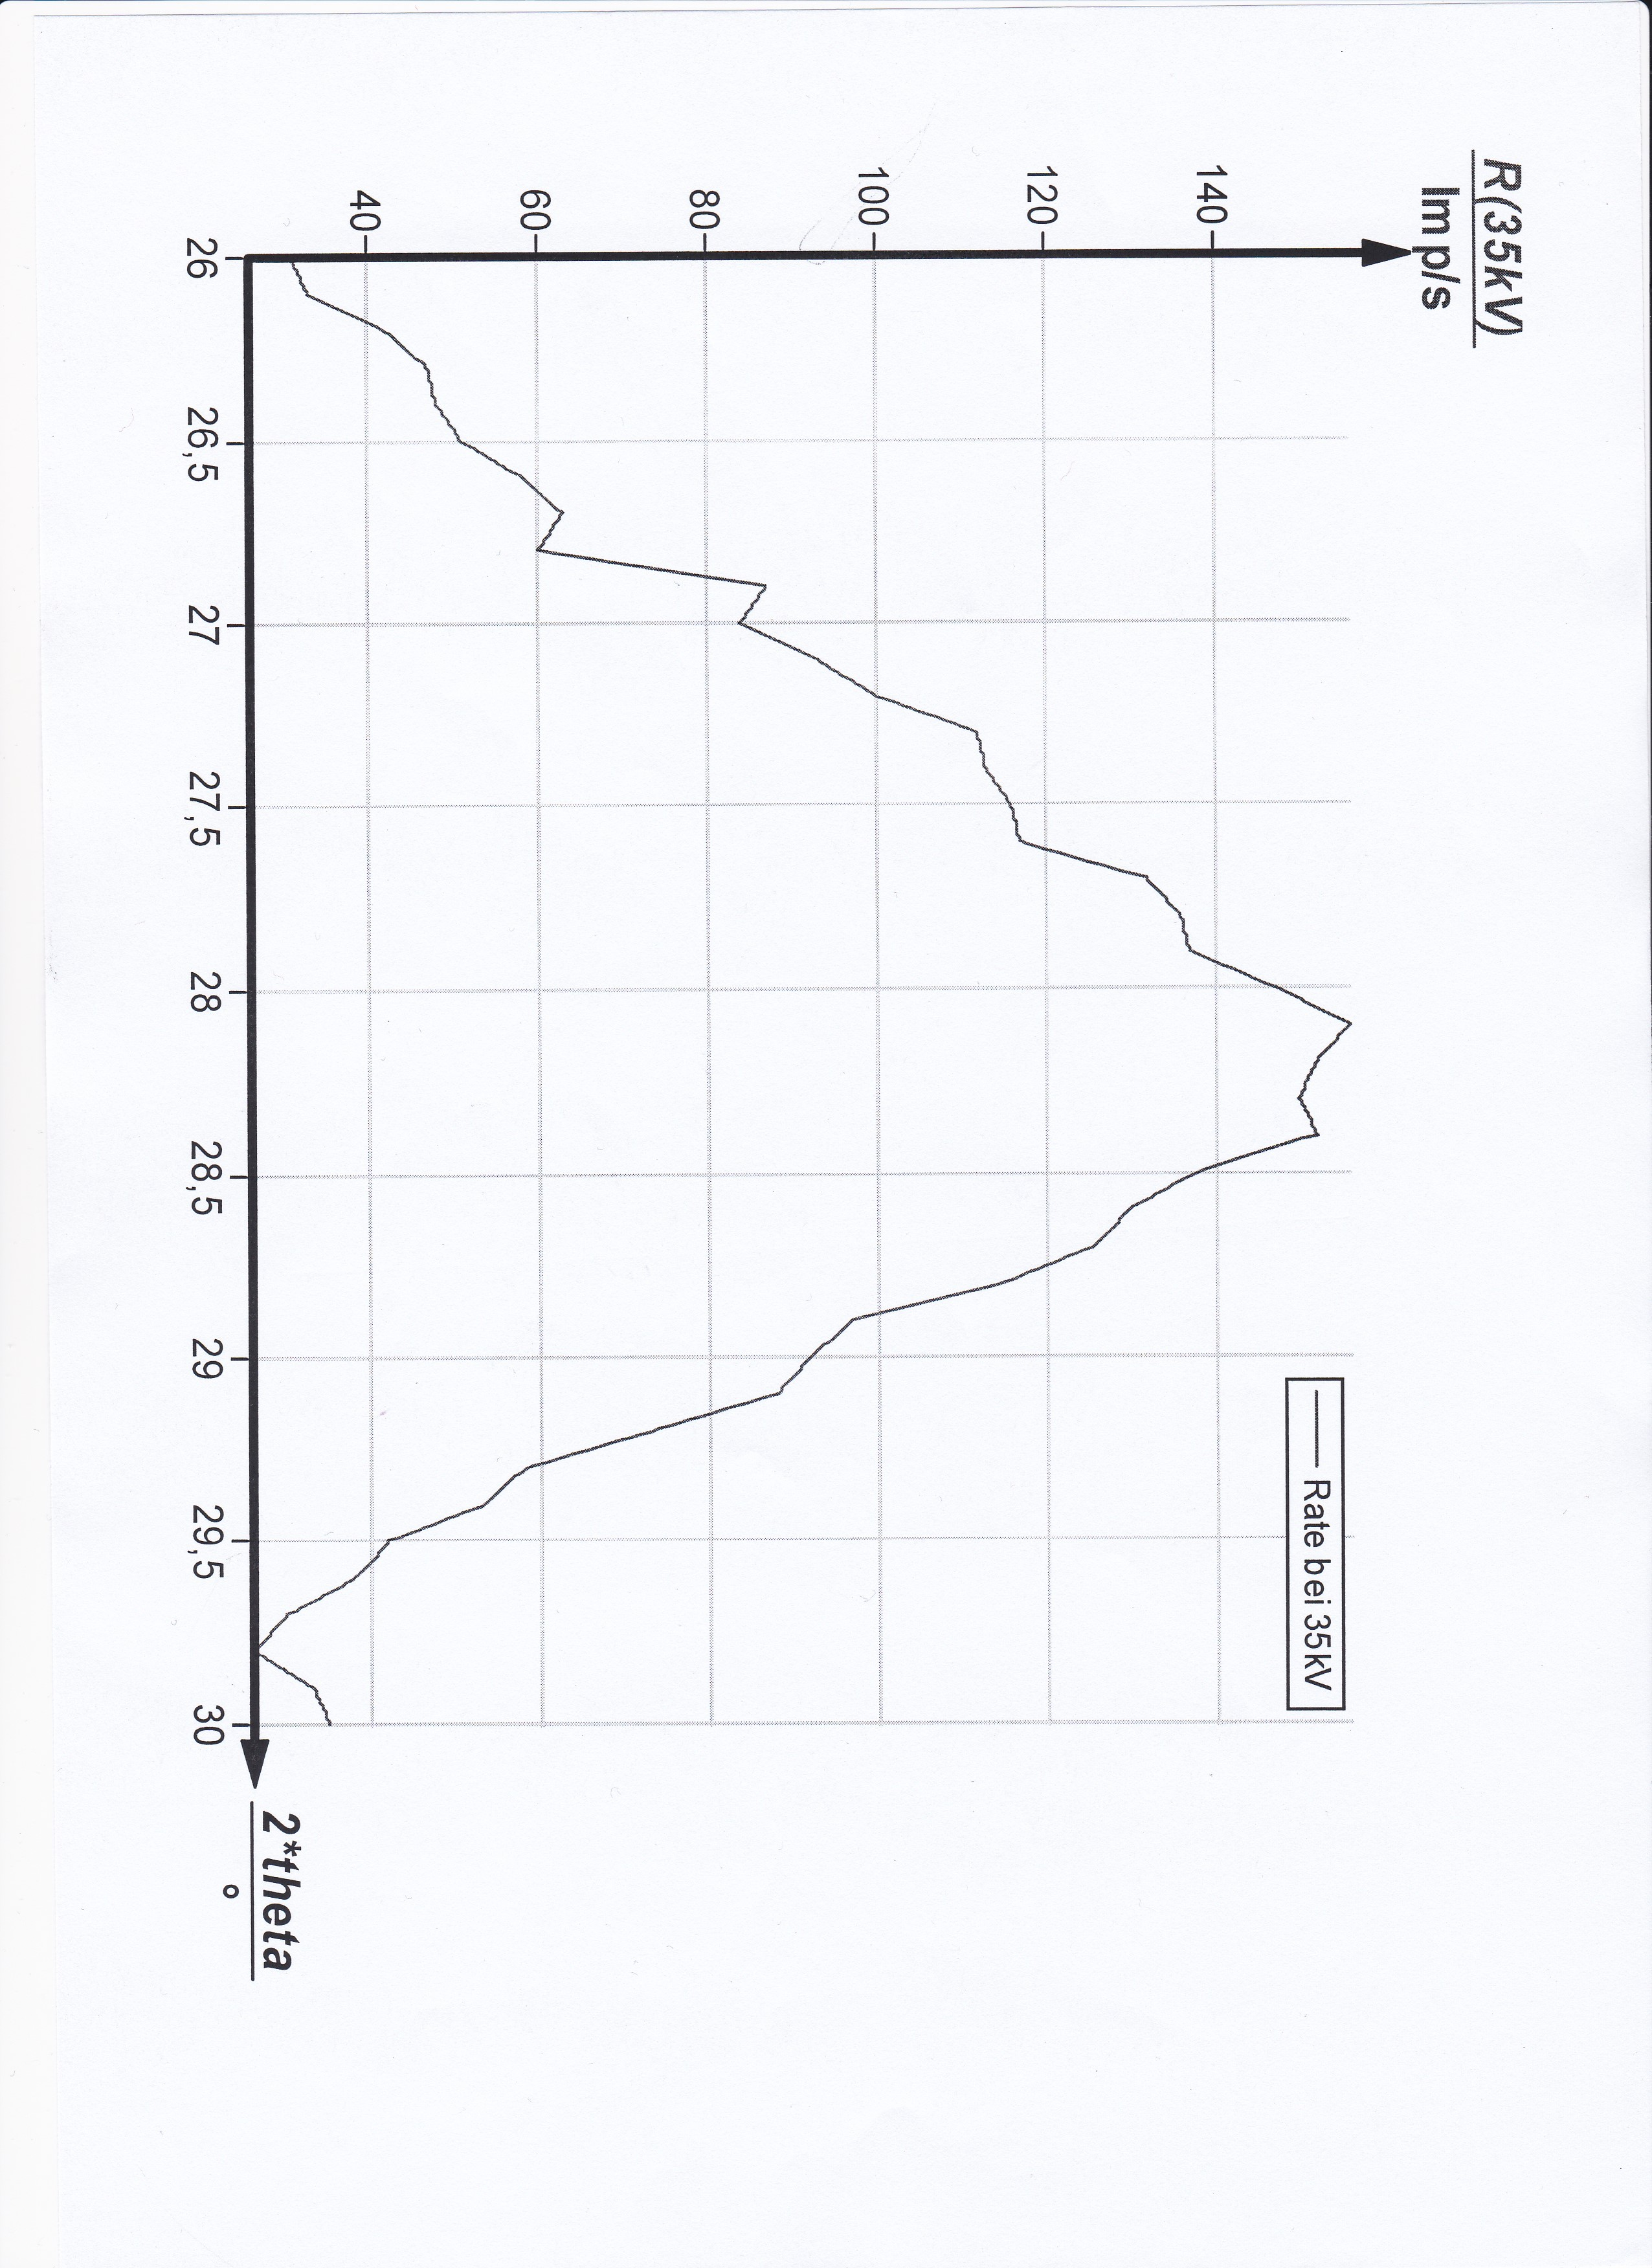
\includegraphics[width=\textwidth]{content/Ueberpruefung.jpg}
  \caption{Überprüfung der Bragg-Bedingung.}
  \label{Bild:1}
\end{figure}
\begin{figure}[p]
  \centering
  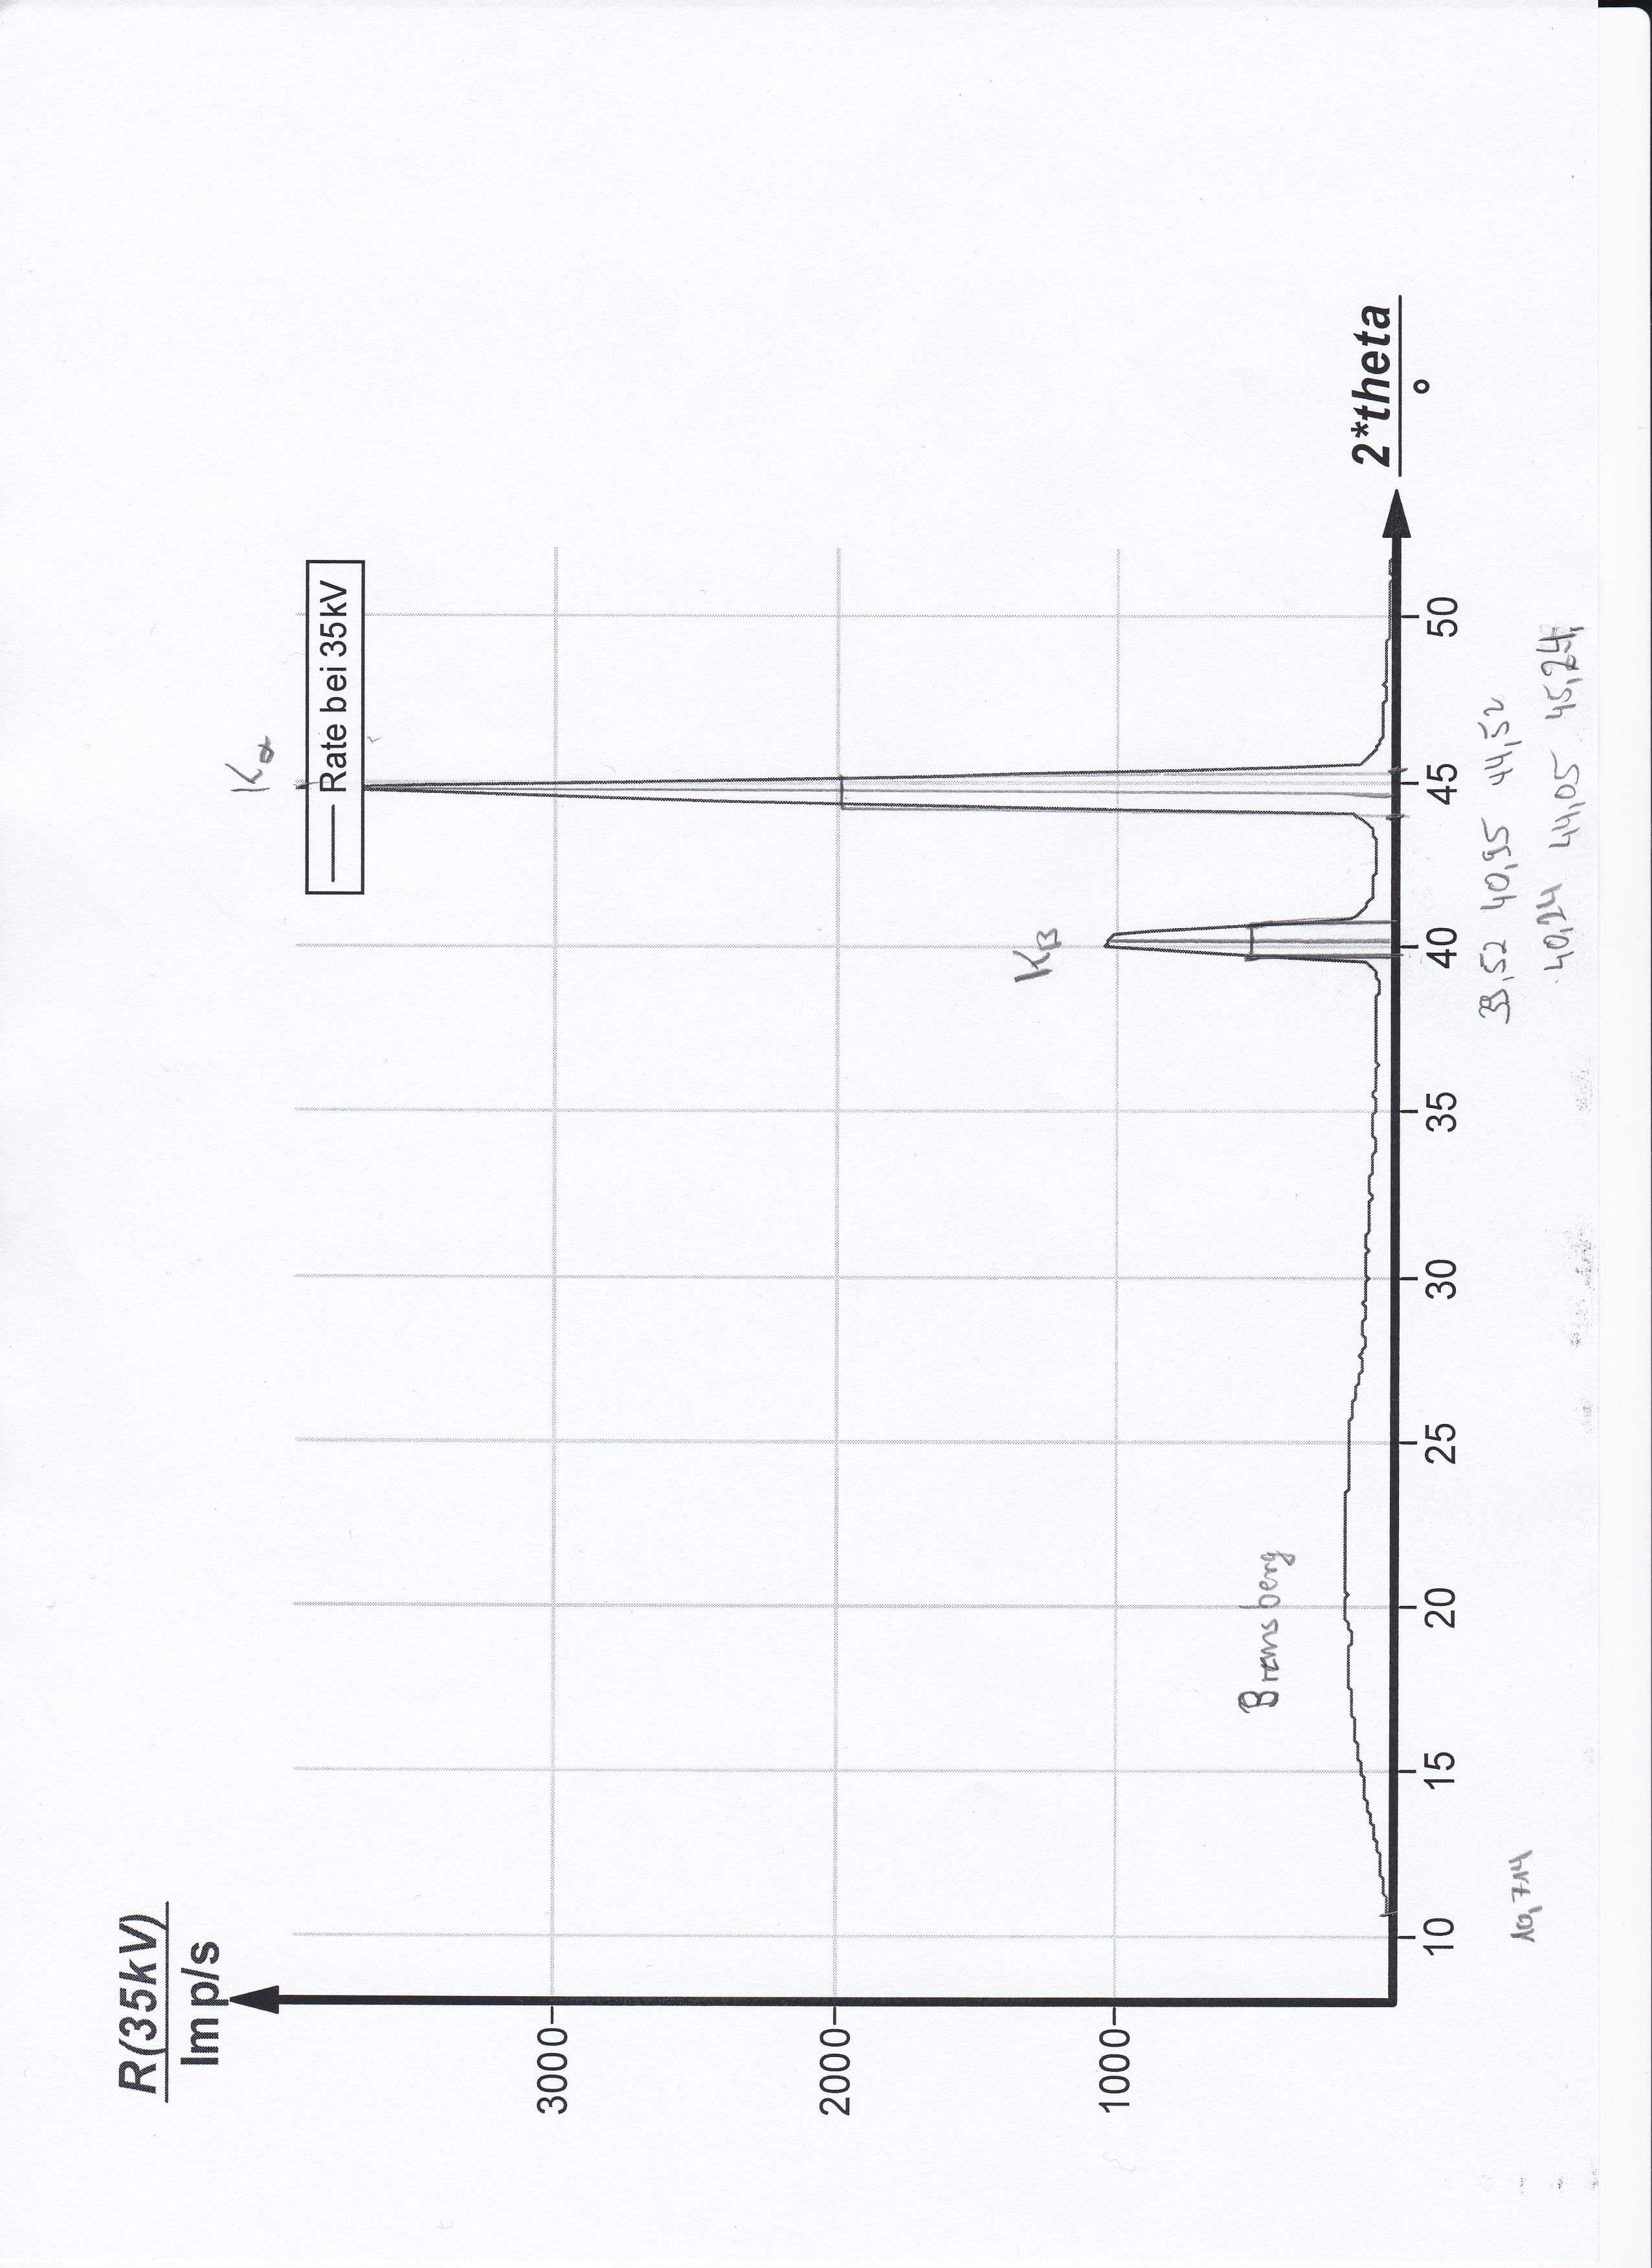
\includegraphics[width=\textwidth]{content/Peaks.jpg}
  \caption{Aufnahme zum Emissionsspektrum der Cu-Röntgenröhre.}
  \label{Bild:2}
\end{figure}
\begin{figure}[p]
  \centering
  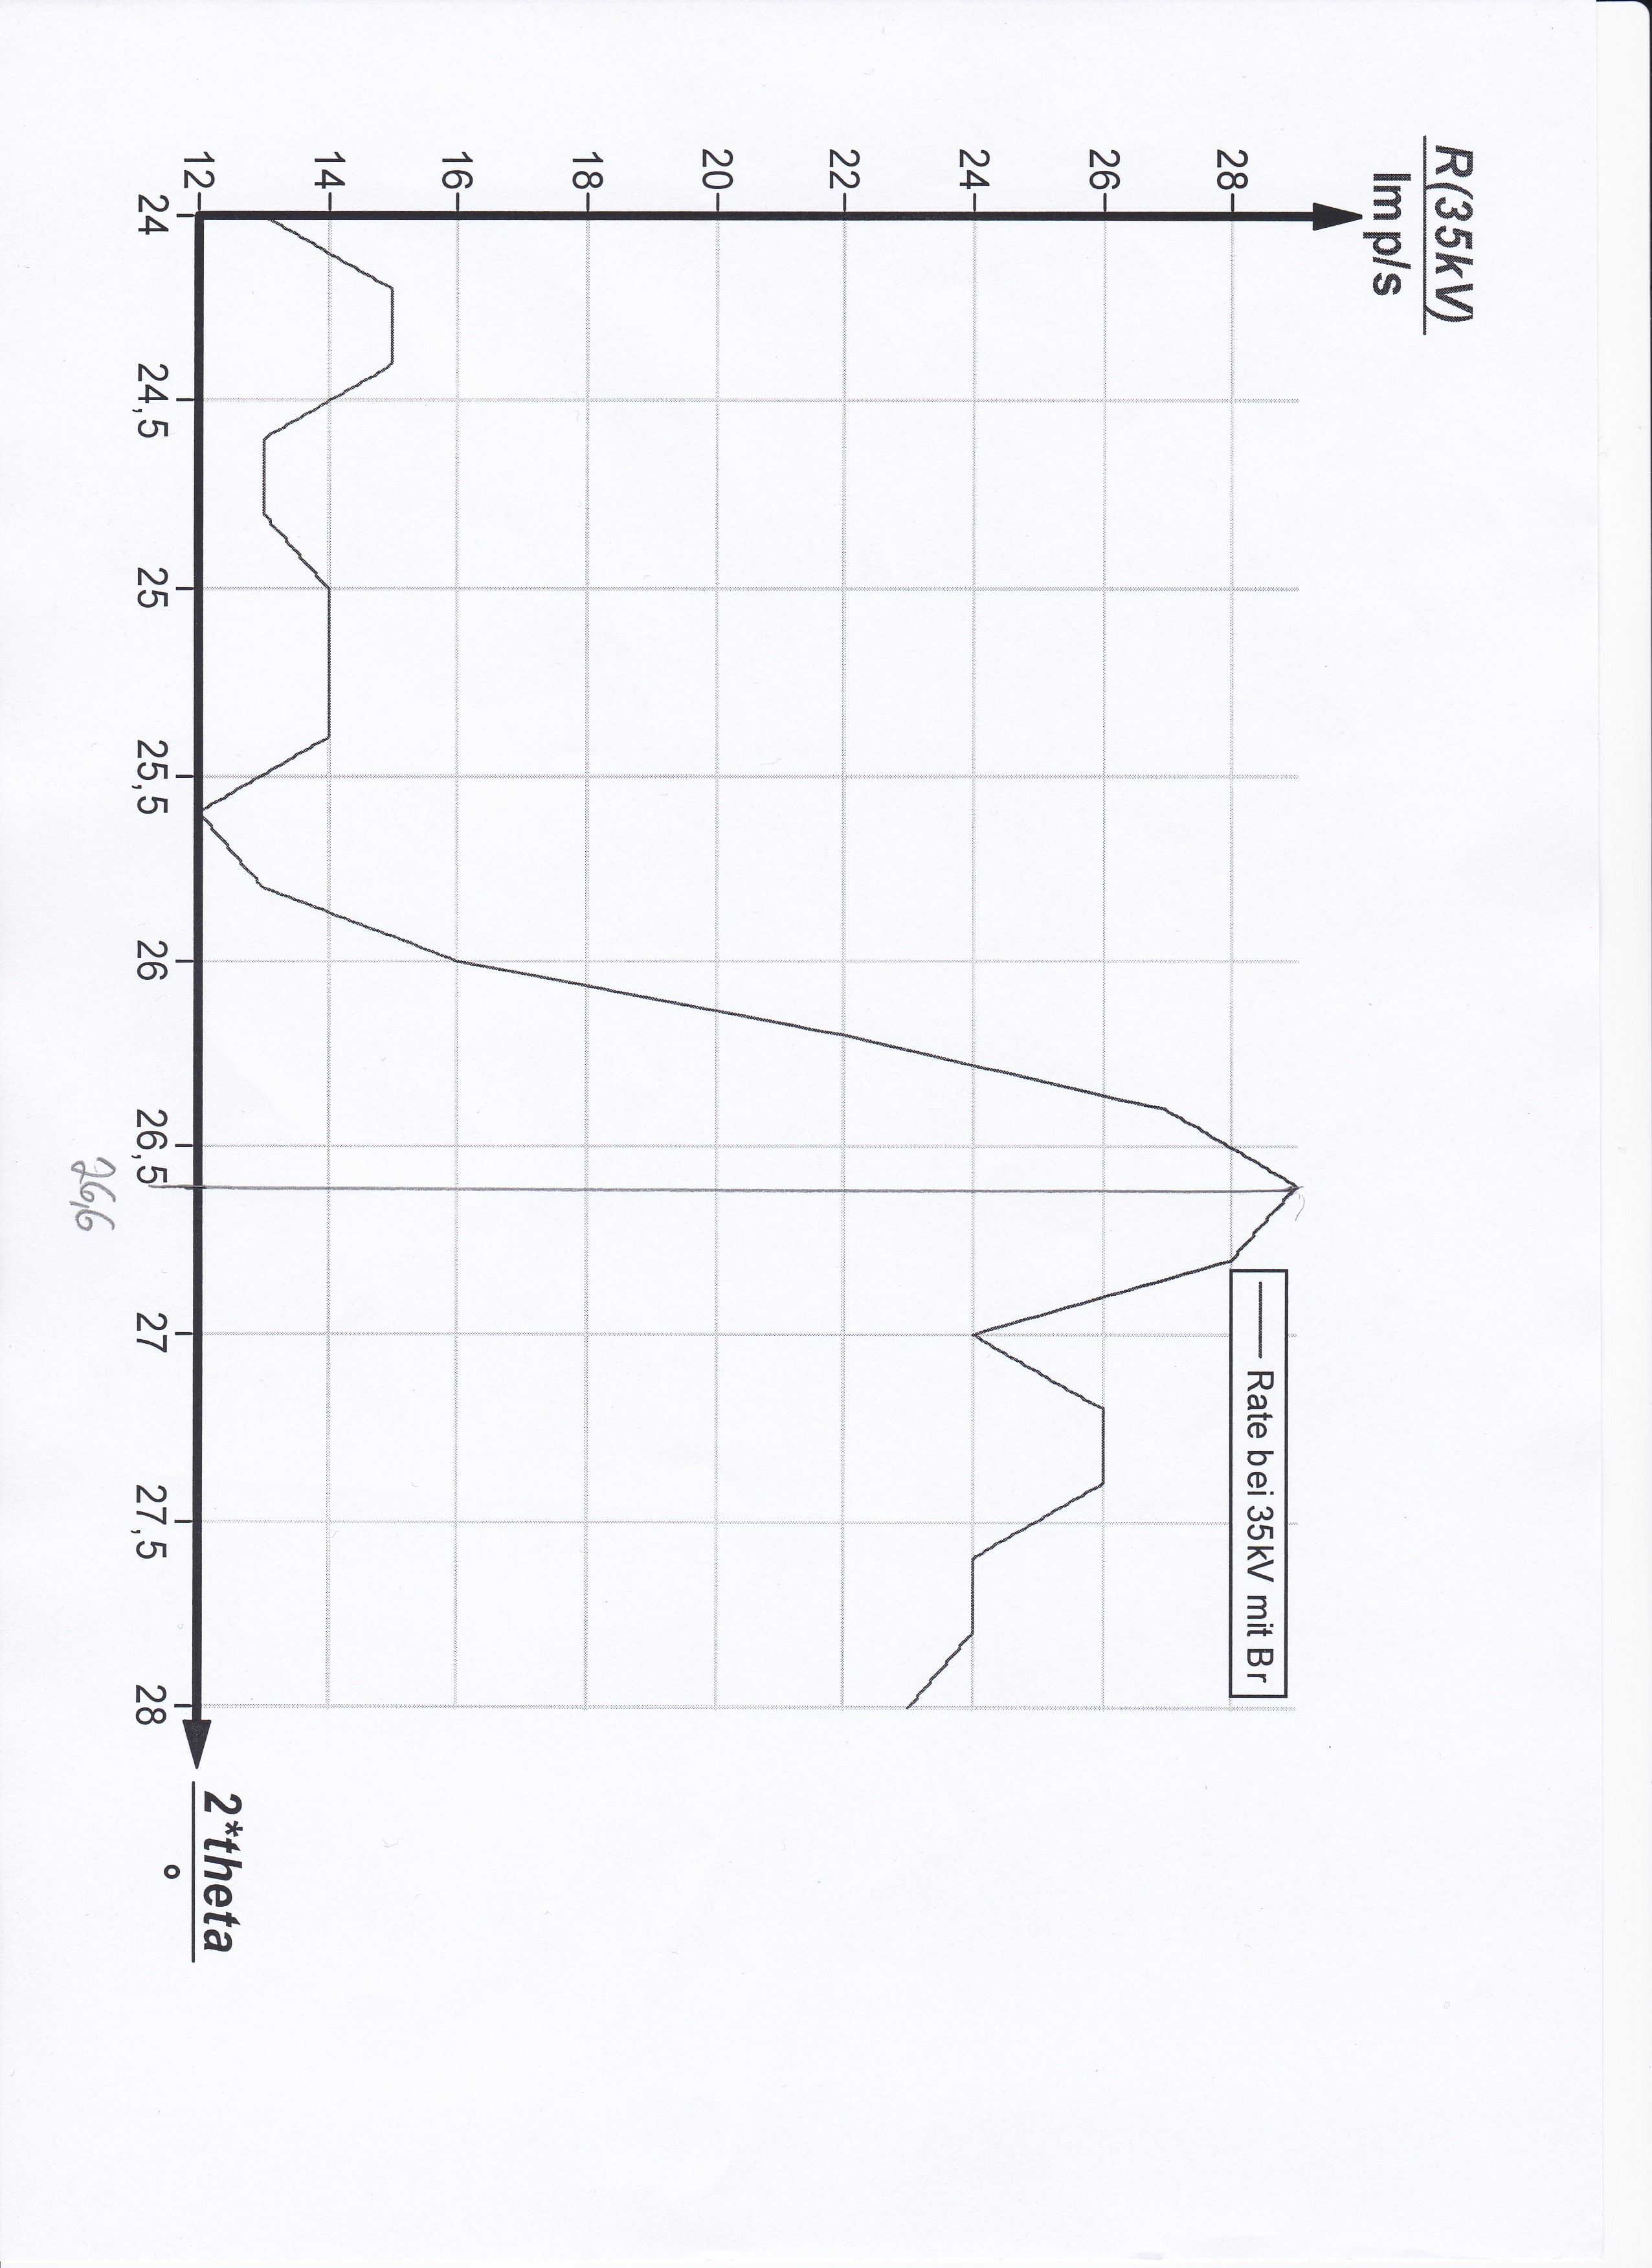
\includegraphics[width=\textwidth]{content/Brom.jpg}
  \caption{Aufnahme mit dem Absorber Brom.}
  \label{Bild:3}
\end{figure}
\begin{figure}[p]
  \centering
  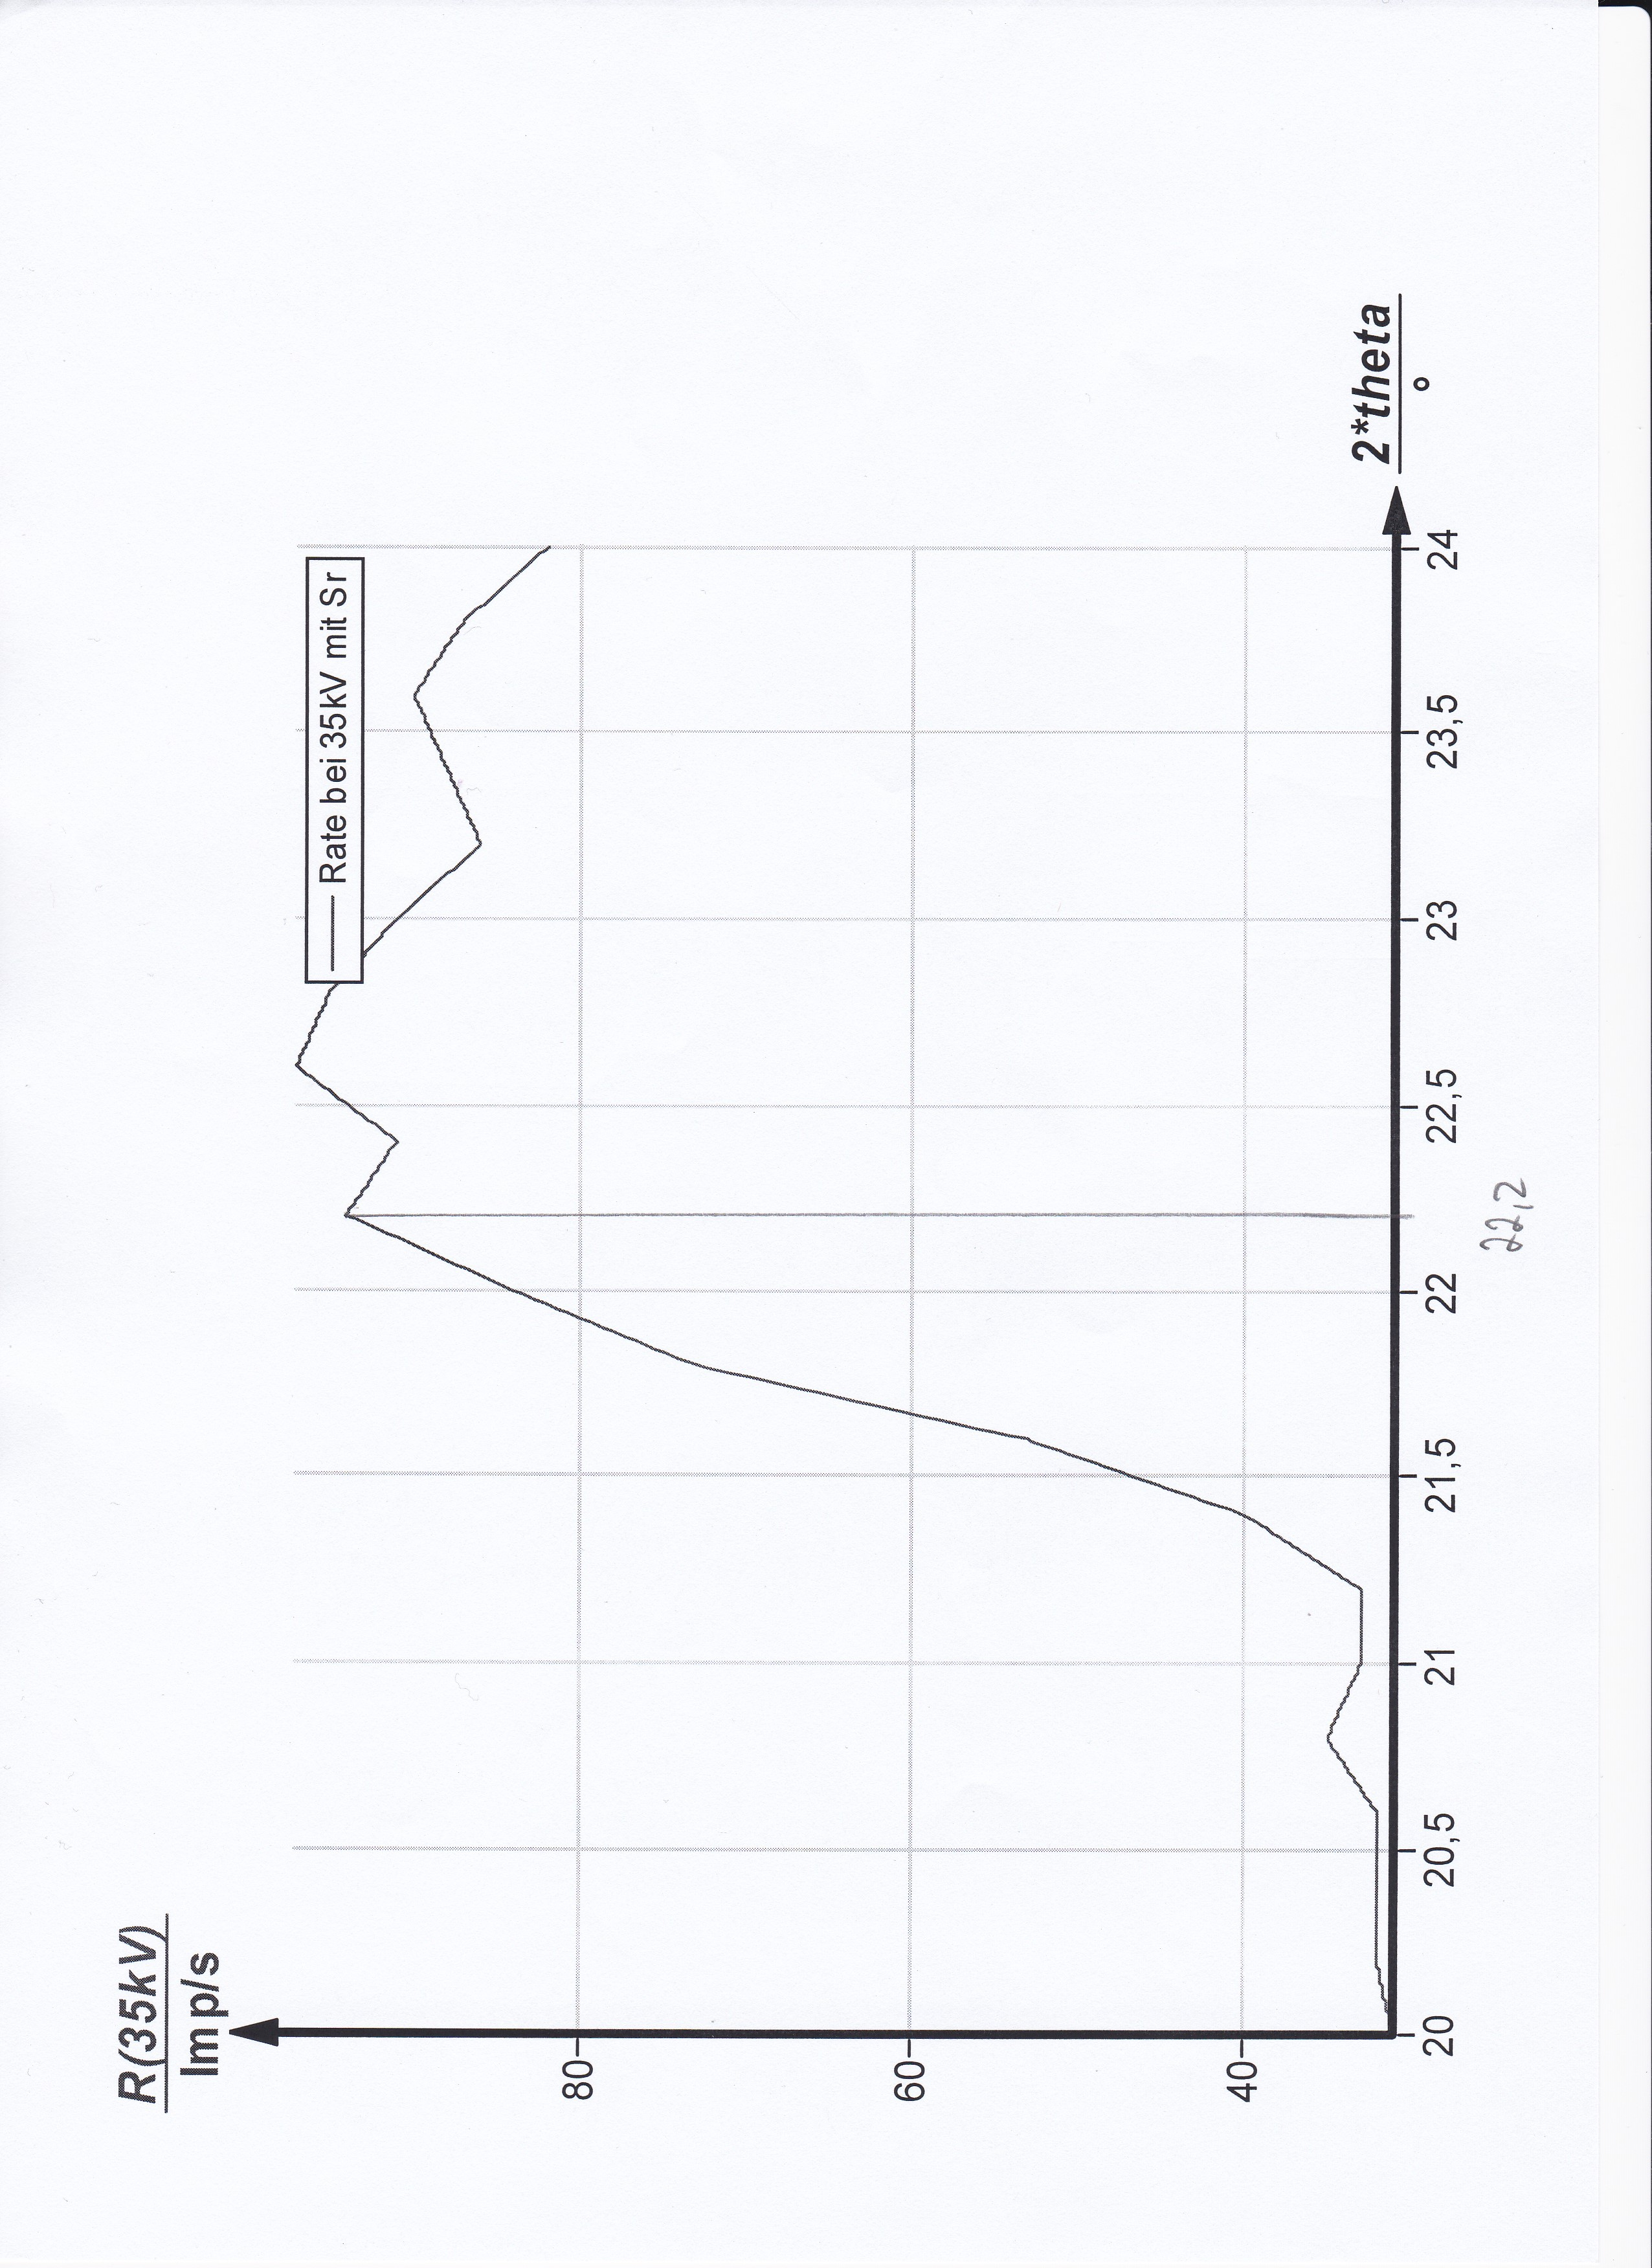
\includegraphics[width=\textwidth]{content/Strontium.jpg}
  \caption{Aufnahme mit dem Absorber Strontium.}
  \label{Bild:4}
\end{figure}
\begin{figure}[p]
  \centering
  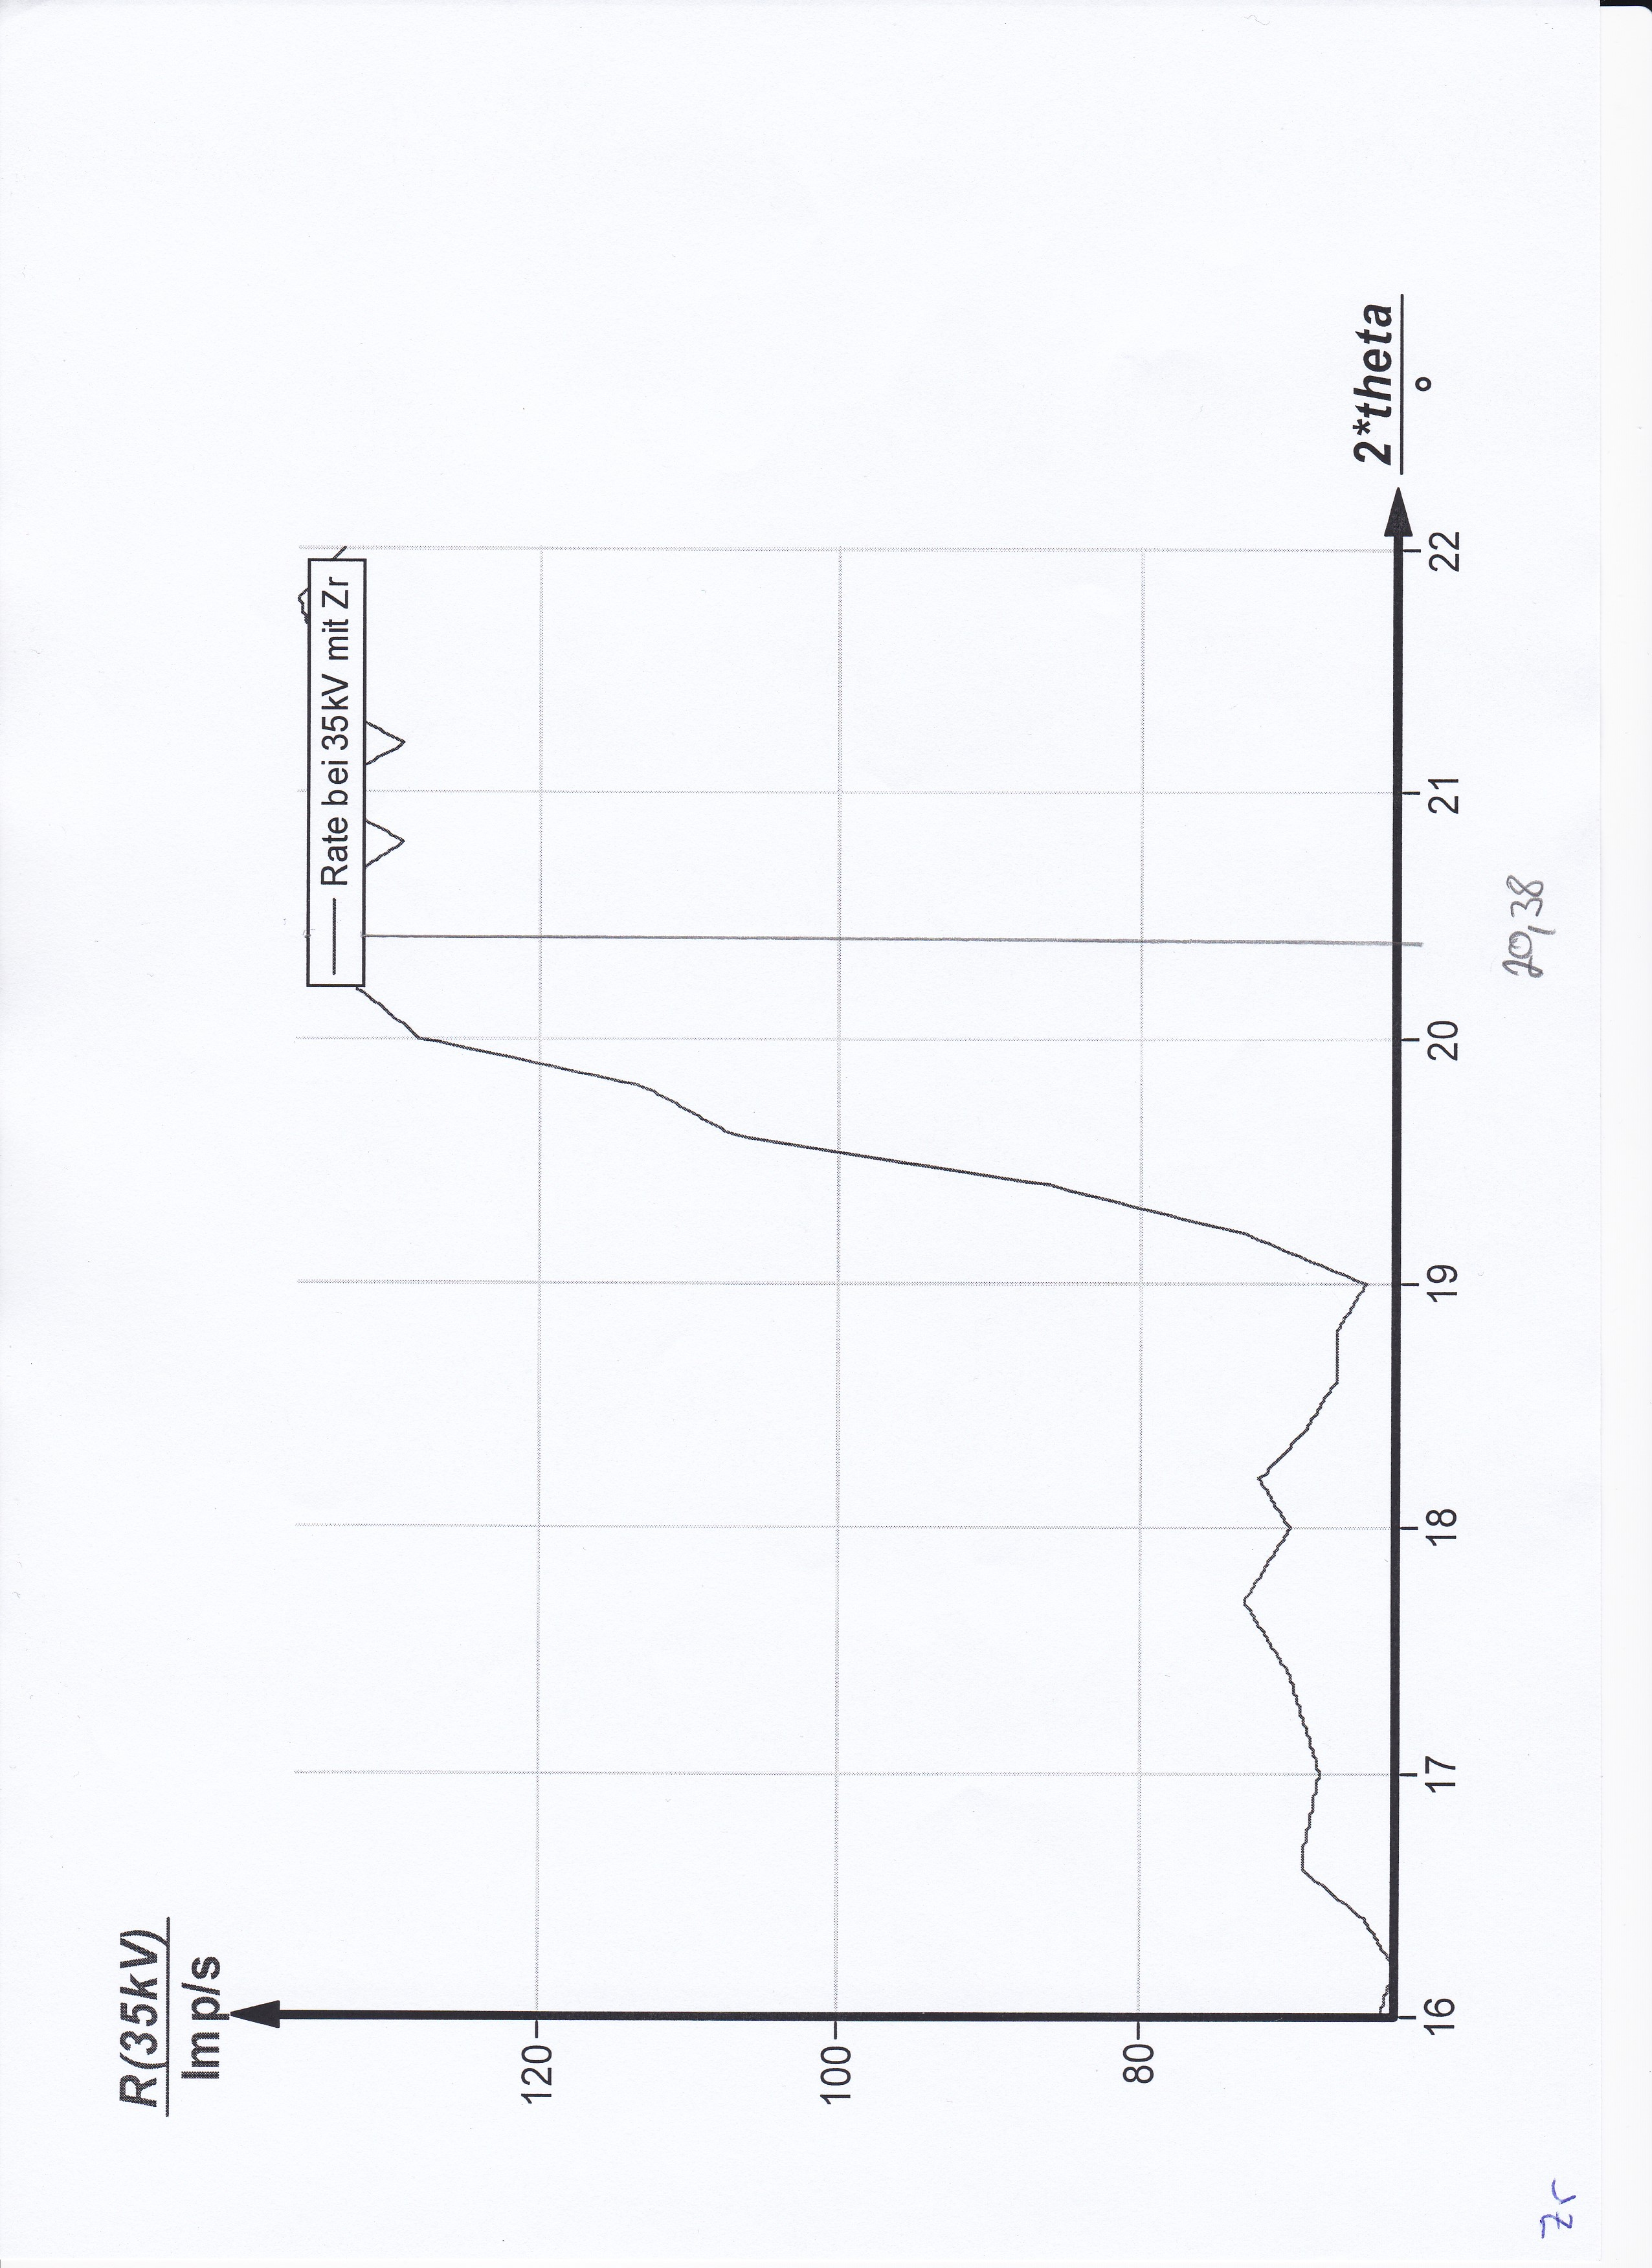
\includegraphics[width=\textwidth]{content/Zirkon.jpg}
  \caption{Aufnahme mit dem Absorber Zirkon.}
  \label{Bild:5}
\end{figure}
\begin{figure}[p]
  \centering
  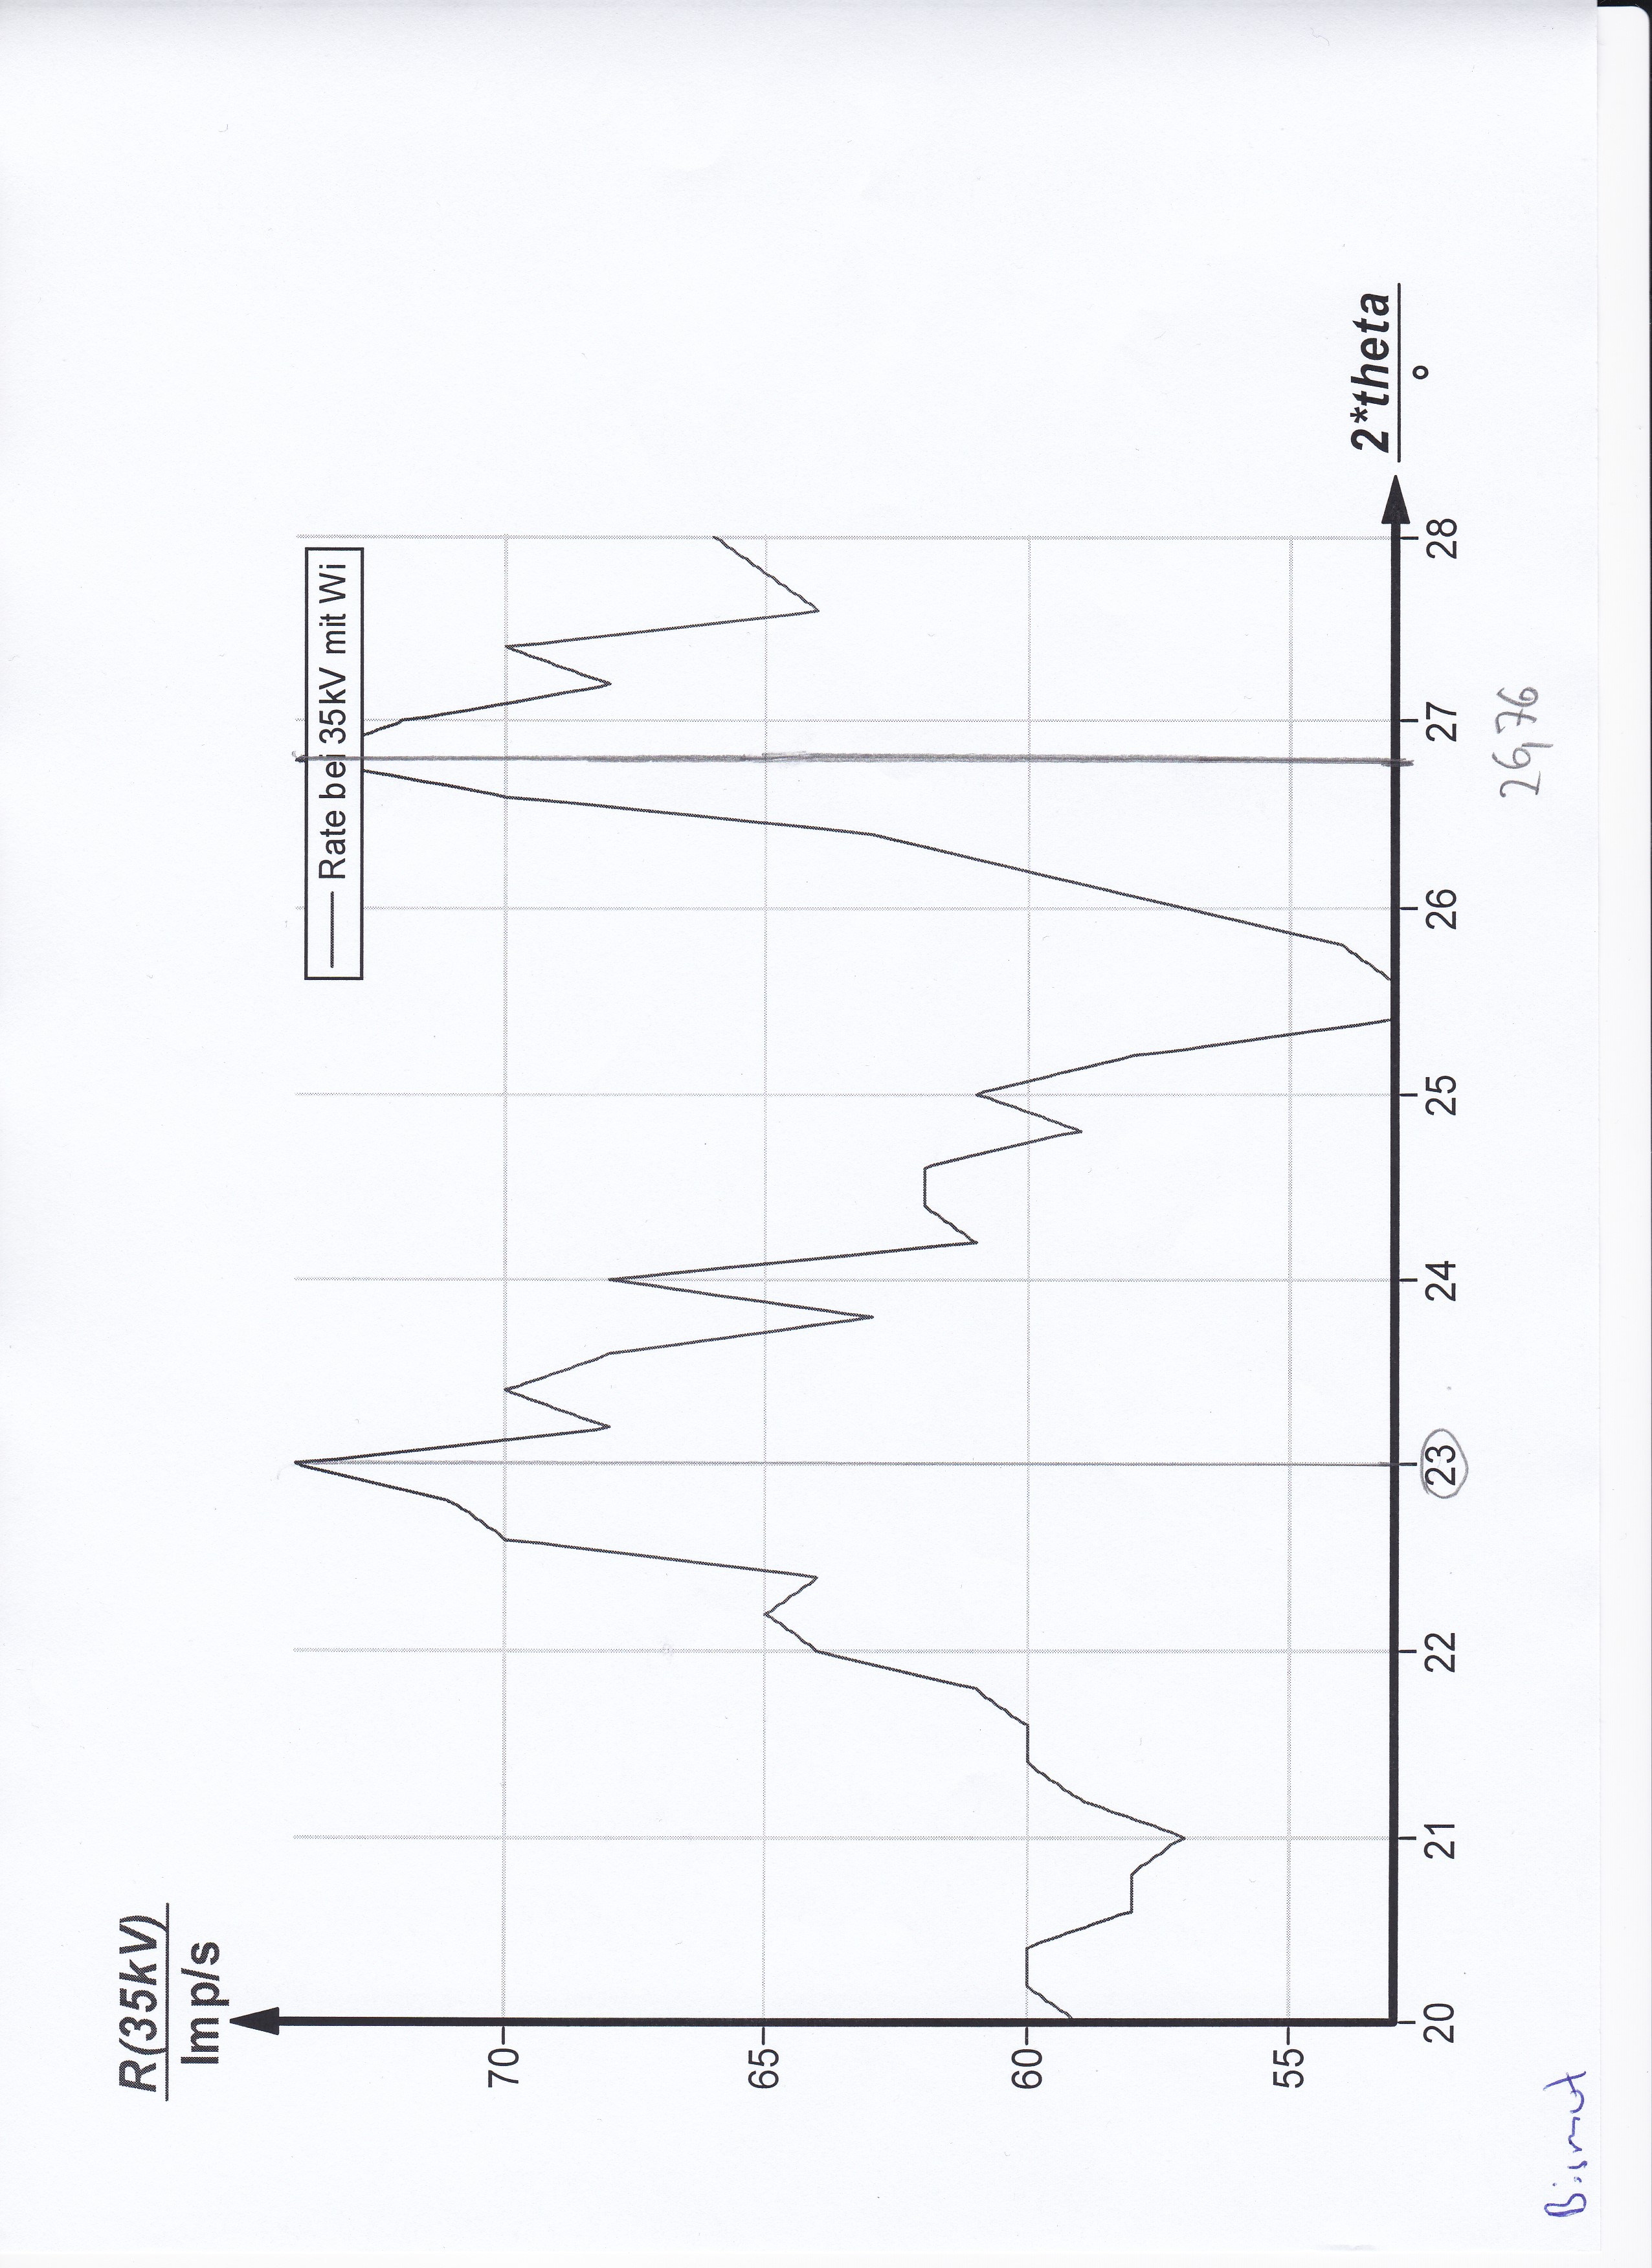
\includegraphics[width=\textwidth]{content/Bismut.jpg}
  \caption{Aufnahme mit dem Absorber Wismut.}
  \label{Bild:6}
\end{figure}
